\subsection{Illustrative visualization: new technology or useless tautology?}
\begin{frame}\frametitle{\emph{Illustrative visualization: new technology or useless tautology?} \cite{1408633}} 
\begin{itemize}
	\item Visualiza��o ilustrativa: Representa��o visual interativa e expressiva, assistida por computador, motivada por ilustra��es tradicionais. Dois n�veis de abstra��o:
	\begin{itemize}
		\item Abstra��es de baixo n�vel: \textbf{como} renderizar as caracter�sticas de interesse (ex: \emph{toon shading}).
		\item Abstra��es de alto n�vel: \textbf{o que} renderizar. (ex: \emph{cutaways} e vistas explodidas).
				\begin{itemize}
					\item Necessitam de informa��es sobre a relev�ncia dos dados.
					\item \emph{Smart visibility techniques} \cite{Viola-05-Smart}.
				\end{itemize}
	\end{itemize}
\end{itemize}	
\end{frame}


\begin{frame}\frametitle{\emph{Illustrative visualization: new technology or useless tautology?} \cite{1408633}} 
	\begin{columns}
		\begin{column}[c]{5cm}
			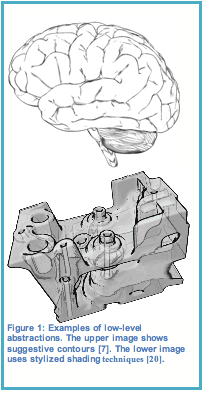
\includegraphics[width=0.6\linewidth]{img/lowlevelabstraction.png}
			\vspace{0cm} 
		\end{column}
		\begin{column}[c]{5cm}
			\begin{overprint}
			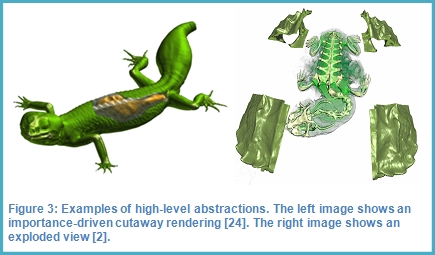
\includegraphics[width=0.8\linewidth]{img/highlevelabstraction.jpg}
			\end{overprint}
		\end{column}
	\end{columns}
\end{frame}



	




				